El objetivo principal del software es el de encontrar soluciones al Problema de la Mínima Dispersión Diferencial lo más cercanas
al óptimo posible y de forma que pueda ejecutarse en un tiempo computacional razonable eficientemente posible. Para conseguir esto
implementamos distintas técnicas de búsqueda, en este caso en concreto utilizando técnicas Greedy y de Búsqueda Local.

\section{Filosofía tras la implementación}

Buscando separar mecanismos de políticas y delimitar claramente las responsabilidades entre clases intentamos generalizar en
distintos módulos lógicos. Después de un proceso iterativo descubrimos que los datos, ya sean de la matriz de distancias
entre puntos o de la solución, son independientes a los algoritmos.
Los algoritmos dependen en estos, pero no al contrario. Por tanto los algoritmos dependen en dos módulos:

    1. Un módulo dedicado a ofrecer mecanismos para importar y acceder a los datos y
    
    2. otro módulo para modificar u obtener información sobre una solución.

Esta separación permite ocultar los detalles acerca de la estructura de datos concreta utilizada tanto como para representar
la información de las distancias entre dos puntos como para representar
la solución al algoritmo. Además, salva a la implementación de este de tener en cuenta todas las operaciones necesarias
para calcular la solución de forma factorizada, pudiendo reutilizarse este código en algoritmos futuros y pudiendo adoptar estructuras
de datos más eficientes en un futuro sin tener por ello que cambiar el código concreto del algoritmo.

Así, los algoritmos describen únicamente las políticas sobre los mecanismos de las estructuras de datos en las que dependen.

\begin{figure}[ht]
    \centering
    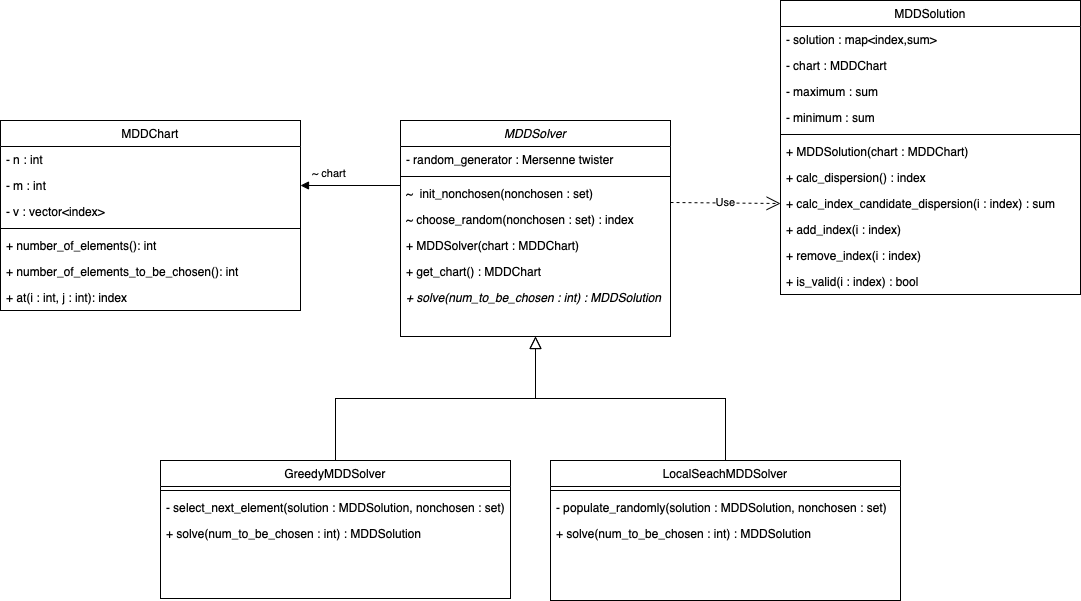
\includegraphics[width=\textwidth]{DiagramaClasesArquitectura.drawio.png}
    \caption{Diagrama de Clases de la solución.}
\end{figure}

\section{Estructuras de datos comunes}

Para representar la matriz que define las distancias entre puntos utilizamos un vector para favorecer la localidad espacial y
temporal de la memoria al realizar un acceso secuencial, como cuando se da el caso cuando necesitamos añadir un punto a una solución.
Gracias a una función constructura podemos leer estos datos de un fichero de texto plano, el cual indica tanto las distancias entre
puntos como el número de puntos existentes en el archivo asi como el número de puntos a seleccionar.

Por otra parte para representar una solución utilizamos un diccionario. Hay alternativas más eficientes, como utilizar un vector binario.
Por ahora esto no nos preocupa, ya que las soluciones se obtienen en un tiempo aceptable aun para instancias grandes del problema y 
al estar abstraidos los mecanismos concretos para actuar sobre la estructura de datos interna concreta que almacena la solución del
algoritmo será fácil de cambiar en un futuro en caso de ser necesario sin afectar por ello a la implementación de los algoritmos. La
interfaz para actuar sobre la solución nos permite añadir y extraer puntos de la solución de la forma más eficiente posible, además
de poder estimar la dispersión de un punto determinado sobre una solución concreta sin tener que añadirlo a la solución en sí. Para
conseguir esto guardamos en el diccionario tanto los puntos escogidos para una solución en concreto como la suma de la distancia desde
el punto al resto de puntos en la solución. En general, estas implementaciones son fruto de unas decisiones de diseño concretas, como la
separación de responsabilidades anteriormente mencionadas, la modificación de un estado únicamente cuando sea necesario, la no pesimización
del código y el cálculo eficiente. Además, minimizamos al máximo la copia y la redundancia de los datos del problema, algoritmo y solución,
ya sea permanente o temporal.

También generalizamos la interfaz de los algoritmos de forma que no sea necesario conocer en tiempo de compilación la implementación
concreta del algoritmo que resuelva el problema.

\section{Aspectos que comparten los distintos algoritmos}

Ambos algoritmos buscan encontrar los puntos pertenecientes al conjunto dado de tal que formen una solución válida y minimicen la dispersión
entre ellos. Por tanto la función objetivo de los algoritmos buscarán encontrar las soluciones tal que $ Disp(Sol^{\prime}) < Disp(Sol) $.

Para tener memoria de los no escogidos en la solución que se devolverá los algoritmos mantienen durante la ejecución del algoritmo un
conjunto de puntos no escogidos que se va actualizando cada vez que se añade, retira o intercambia un punto de la solución.

\section{Añadir y eliminar puntos de la solución. Cálculo de la dispersión de una solución o posible solución}

Como comentamos superficialmente en secciones anteriores la inserción y eliminación de un punto de la solución está implementada de tal
forma que consuma la cantidad mínima de recursos en tiempo, consiguiendo realizar ambas en orden $ \Theta(m) $, siendo $ m $ el 
número de puntos en la solución después de insertar o antes de eliminar.

Para conseguir esto seguimos el algoritmo definido en pseudocódigo en la función \texttt{inserta\_punto\_en\_solucion}, el cual es también bastante parecido
a la función \texttt{elimina\_punto\_de\_solucion}.

\begin{minipage}{\textwidth}
\begin{lstlisting}[mathescape=true,caption={Definición en pseudocódigo de las funciones que permiten añadir y eliminar puntos a una solución.},captionpos=b]
def suma_distancias_desde_un_punto_hasta_los_puntos_de_una_solucion(v, solucion):
    sum = 0
    por cada punto p en solucion:
        sum = sum + distancia(v, p)
    devuelve sum

def inserta_punto_en_solucion(v, solucion):
    si v $ \in $ solucion:
        aborta

    por cada punto p en solucion:
        p.suma_distancias = p.suma_distancias + distancia(v, p)
    
    v.suma_distancias =
        suma_distancias_desde_un_punto_hasta_los_puntos_de_una_solucion(v, solucion)
    solucion.inserta(v)

def elimina_punto_de_solucion(v, solucion):
    si v $ \notin $ solucion:
        aborta
    
    por cada punto p en solucion:
        p.suma_distancias = p.suma_distancias - distancia(v, p)
    
    solucion.elimina(v)
\end{lstlisting}
\end{minipage}

Además, declaramos y definimos una función con nombre \texttt{calcula\_dispersion\_de\_punto\_candidato} para calcular
la dispersión que tendríamos si añadiésemos un determinado punto a la solución.

\begin{minipage}{\textwidth}
\begin{lstlisting}[mathescape=true,caption={Definición de la función que nos permite calcular la dispersión de un punto candidato si perteneciese a una solución.},captionpos=b]
def calcula_dispersion_de_punto_candidato(v, solucion):
    min = $ + \infty $
    max = $ 0 $
    sum_v =
        suma_distancias_desde_un_punto_hasta_los_puntos_de_una_solucion(v, solucion)
    max = $ max $(max, sum_v)
    min = $ min $(min, sum_v)

    por cada punto p en solucion:
        sum_punto_sol = p.suma_distancias + distancia(v, p)
        max = $ max $(max, sum_punto_sol)
        min = $ min $(min, sum_punto_sol)
    
    devuelve max - min
\end{lstlisting}
\end{minipage}

\section{Selección de elementos aleatorios}

Para generar números aleatorios hemos utilizado un generador pseudo-aleatorio de tipo Mersenne Twister, inicializado con una semilla.
Para seleccionar un elemento perteneciente a un conjunto hemos utilizado un generador aleatorio que devuelve valores en una distribución uniforme
el cual utiliza como motor el generador mencionado anteriormente.